\documentclass[UTF8]{report}
\usepackage{amsmath}
\usepackage{cite}
\usepackage{algorithm}
\usepackage{algorithmicx}
\usepackage{algpseudocode}
\usepackage{lipsum,float}
\usepackage{geometry}
\usepackage{graphicx} %use graph format
\usepackage{epstopdf}
\usepackage{float}
\usepackage{subfigure}
\usepackage{listings}
\usepackage{color}
\definecolor{dkgreen}{rgb}{0,0.6,0}
\definecolor{gray}{rgb}{0.5,0.5,0.5}
\definecolor{mauve}{rgb}{0.58,0,0.82}
\lstset{breaklines}%自动将长的代码行换行排版
\lstset{ %
extendedchars=false,            % Shutdown no-ASCII compatible
language=Matlab,                % choose the language of the code
basicstyle=\footnotesize\tt,    % the size of the fonts that are used for the code
tabsize=3,                            % sets default tabsize to 3 spaces
numbers=left,                   % where to put the line-numbers
numberstyle=\tiny,              % the size of the fonts that are used for the line-numbers
stepnumber=1,                   % the step between two line-numbers. If it's 1 each line
                                % will be numbered
numbersep=5pt,                  % how far the line-numbers are from the code   %
keywordstyle=\color[rgb]{0,0,1},                % keywords
commentstyle=\color[rgb]{0.133,0.545,0.133},    % comments
stringstyle=\color[rgb]{0.627,0.126,0.941},      % strings
backgroundcolor=\color{white}, % choose the background color. You must add \usepackage{color}
showspaces=false,               % show spaces adding particular underscores
showstringspaces=false,         % underline spaces within strings
showtabs=false,                 % show tabs within strings adding particular underscores
frame=single,                 % adds a frame around the code
captionpos=b,                   % sets the caption-position to bottom
breaklines=true,                % sets automatic line breaking
breakatwhitespace=false,        % sets if automatic breaks should only happen at whitespace
title=\lstname,                 % show the filename of files included with \lstinputlisting;
                                % also try caption instead of title
mathescape=true,escapechar=?    % escape to latex with ?..?
escapeinside={\%*}{*)},         % if you want to add a comment within your code
%columns=fixed,                  % nice spacing
%morestring=[m]',                % strings
%morekeywords={%,...},%          % if you want to add more keywords to the set
%    break,case,catch,continue,elseif,else,end,for,function,global,%
%    if,otherwise,persistent,return,switch,try,while,...},%
}
\geometry{a4paper,left=2.5cm,right=2.5cm,top=2.5cm,bottom=2.5cm}
\renewcommand{\bibname}{Reference}

\title{\Huge \textbf{PCP Problem And Image Deblurring}}
\author{Jingxiang Wu}
\date{\today}
\makeatletter
\newenvironment{breakablealgorithm}
  {% \begin{breakablealgorithm}
   \begin{center}
     \refstepcounter{algorithm}% New algorithm
     \hrule height.8pt depth0pt \kern2pt% \@fs@pre for \@fs@ruled
     \renewcommand{\caption}[2][\relax]{% Make a new \caption
       {\raggedright\textbf{\ALG@name~\thealgorithm} ##2\par}%
       \ifx\relax##1\relax % #1 is \relax
         \addcontentsline{loa}{algorithm}{\protect\numberline{\thealgorithm}##2}%
       \else % #1 is not \relax
         \addcontentsline{loa}{algorithm}{\protect\numberline{\thealgorithm}##1}%
       \fi
       \kern2pt\hrule\kern2pt
     }
  }{% \end{breakablealgorithm}
     \kern2pt\hrule\relax% \@fs@post for \@fs@ruled
   \end{center}
  }
\makeatother
\begin{document}\large
\maketitle
\tableofcontents
\chapter{PCP Problem And Several Algorithms For Solving RPCA}
The problem of image deblurring can be regarded as the decomposition of a matrix into a low-rank matrix and a sparse matrix. The premise is that the original image is low-rank, or its singular value distribution is reasonable, in which each non-zero element of the sparse matrix is almost the same as that of the low-rank matrix.
\section{The Principal Component Pursuit Problem}

Let A is a given low-rank matrix with sparse noise, which can be decomposed into the sum of L and S. The goal is to reduce the rank of matrix L and the number of elements of matrix S, i.e.:
\[\begin{array}{l}
\min_{L,S}\{ rank(L),{\left\| S \right\|_0}\}\\
s.t.     A = L + S
\end{array}\]

We can add a balance factor \(\lambda \) to make the two relatively balanced, and notice that the rank of the matrix is in the order of magnitude of \(O(\sqrt n )\), and the element of the sparse matrix is in the order of magnitude of \(O(n)\). Generally, \(\lambda \) is set to be \(\frac{1}{{\sqrt {mn} }}\).
\[\begin{array}{l}
\min_{L,S}(rank(L) + \lambda {\left\| S \right\|_0})\\
s.t.     A = L + S
\end{array}\]

This problem is called Principal Component Pursuit.Considering that the rank sum matrix 0 norm cannot be derived, we relax this problem into a convex optimization problem, which is also called Robust Principal Component Analysis.
\[\begin{array}{l}
\min ({\left\| L \right\|_*} + \lambda {\left\| S \right\|_1})\\
s.t.A = L + S
\end{array}\]

\({\left\| L \right\|_*}\) is the kernel norm of a matrix, the sum of all singular values. Then we introduce three algorithms for RPCA.
\section{The Iterative Thresholding Algorithm}
At first, we introduce two operators of matrices, which are the optimal solutions of a class of optimization problems.

The optimal solution of the optimization problem \(\min_X (\varepsilon {\left\| X \right\|_1} + \left\| {X - Q} \right\|_F^2/2)\) is \(X = {S_\varepsilon }(Q)\), the element of matrix is \({S_\varepsilon }{(Q)_{ij}} = \max (\left| {{q_{ij}}} \right| - \varepsilon ,0)*{\mathop{\rm sgn}} ({q_{ij}})\).

The optimal solution of the optimization problem \(\min_X (\varepsilon {\left\| X \right\|_*} + \left\| {X - Q} \right\|_F^2/2)\) is \(X = {D_\varepsilon }(Q)\). Let the singular value decomposition of matrix Q be \(Q = U\Sigma {V^T}\),  and we can get: \({D_\varepsilon }(Q) = U{S_\varepsilon }(\Sigma ){V^T}\)

Considering the regularization of RPCA problem, we can get a new optimization problems.
\[\begin{array}{l}
\min ({\left\| L \right\|_*} + \lambda {\left\| S \right\|_1} + \mu (\left\| L \right\|_F^2 + \left\| S \right\|_F^2)/2)\\
s.t.A = L + S
\end{array}\]

We can get the following iterative algorithm based on the above formula.\cite{IT}
\renewcommand{\algorithmicrequire}{\textbf{Input:}}
\renewcommand{\algorithmicensure}{\textbf{Output:}}
\begin{breakablealgorithm}
  \caption{Iterative Thresholding}
  \label{alg::Iterative Thresholding}
  \begin{algorithmic}[1]
    \Require $A$: a matrix A and Maximum number of iterations iter times
    \Ensure $L$: a low rank matrix; $S$: a sparse matrix
    \State \(\lambda  = \frac{1}{{\sqrt {mn} }}\)
    \State \(\tau  = 0.9{\left\| A \right\|_2}\)
    \State \(Y=0\)
    \State Give \(\delta_0\)
    \For{$k=1$ to iter times}
        \State\({L_k} = {D_\tau }({Y_{k - 1}})\)
        \State\({S_k} = {S_{\lambda \tau }}({Y_{k - 1}})\)
        \State\({Y_k} = {Y_{k - 1}} + {\delta _k}(D - {L_k} - {S_k})\)
        \State update \(\delta_k\)
    \EndFor
  \end{algorithmic}
\end{breakablealgorithm}
\section{The Accelerated Proximal Gradient Algorithm}
According to the slow iteration of the IT algorithm, people improve it and get the following algorithm, which is called Accelerated Proximal Gradient:
\renewcommand{\algorithmicrequire}{\textbf{Input:}}
\renewcommand{\algorithmicensure}{\textbf{Output:}}
\begin{breakablealgorithm}
  \caption{Accelerated Proximal Gradient}
  \label{alg::Accelerated Proximal Gradient}
  \begin{algorithmic}[1]
    \Require $A$: a matrix A and Maximum number of iterations iter times
    \Ensure $L$: a low rank matrix; $S$: a sparse matrix
    \State \({L_1} = {L_0} = 0,{S_1} = {S_0} = 0,{t_1} = {t_0} = 1\)
    \State \(\lambda  = \frac{1}{{\sqrt {mn} }}\)
    \State \(Lf=2\)
    \State \(\tau  = 0.9{\left\| A \right\|_2}\)
    \State Give \(\mu_0\)
    \For{$k=1$ to iter times}
        \State\(Y_k^L = {L_k} + \frac{{{t_{k - 1}} - 1}}{{{t_k}}}({L_k} - {L_{k - 1}})\)
        \State\(Y_k^S = {S_k} + \frac{{{t_{k - 1}} - 1}}{{{t_k}}}({E_k} - {E_{k - 1}})\)
        \State\({L_k} = {D_{\frac{{{\mu _k}}}{{{L_f}}}}}(Y_k^L + \frac{1}{2}(A - Y_k^L - Y_k^S))\)
        \State\({S_k} = {S_{\frac{{\lambda {\mu _k}}}{{{L_f}}}}}(Y_k^S + \frac{1}{2}(A - Y_k^L - Y_k^S))\)
        \State\({\mu _{k + 1}} = \max (\eta {\mu _k},\overline \mu  )\)
        \State\({t_{k + 1}} = \frac{{1 + \sqrt {1 + 4t_k^2} }}{2}\)
    \EndFor
  \end{algorithmic}
\end{breakablealgorithm}
\section{The Augmented Lagrange Multipliers Algorithm}

Using augmented Lagrangian multiplier method to solve PCP problem and constructing augmented Lagrangian Function :\cite{ALM}

\[L(L,S,Y,\mu ) = {\left\| L \right\|_*} + \lambda {\left\| S \right\|_1} + \left\langle {\left. {Y,A - L - S} \right\rangle  + } \right.\mu \left\| {A - L - S} \right\|_F^2/2\]

Before each update of the auxiliary matrix Y, we need to update L and S repeatedly in a cycle to converge. In order to improve the speed, people propose to update L and S only once, which is called inexact ALM:

\renewcommand{\algorithmicrequire}{\textbf{Input:}}
\renewcommand{\algorithmicensure}{\textbf{Output:}}
\begin{breakablealgorithm}
  \caption{Accelerated Proximal Gradient}
  \label{alg::Accelerated Proximal Gradient}
  \begin{algorithmic}[1]
    \Require $A$: a matrix A and Maximum number of iterations iter times
    \Ensure $L$: a low rank matrix; $S$: a sparse matrix
    \State \(\lambda  = \frac{1}{{\sqrt {mn} }}\)
    \State \(Y_0=S_0=0\)
    \State Give \(\mu_0\)
    \For{$k=1$ to iter times}
        \State\({L_{k + 1}} = {D_{\frac{1}{{{\mu _k}}}}}(A - {S_k} + \mu _k^{ - 1}{Y_k})\)
        \State\({S_{k + 1}} = {S_{\frac{\lambda }{{{\mu _k}}}}}(A - {L_{k + 1}} + \mu _k^{ - 1}{Y_k})\)
        \State\({Y_{k + 1}} = {Y_k} + {\mu _k}(A - {L_{k + 1}} - {S_{k + 1}})\)
        \State update \(\mu_k\)
    \EndFor
  \end{algorithmic}
\end{breakablealgorithm}
\chapter{Image Deblurring and Separation Testing}
The relaxation problem of PCP problem can separate the low-rank matrix L and the sparse noise matrix S under the condition that the singular value distribution of the original matrix L is reasonable. We can apply this technology to the scene of repairing the image and removing high-intensity noise from the image. The premise is that the image should be relatively low-rank. Otherwise, we can choose a part of the image for this operation.

First, We choose several background maps, draw some stains on them, and then use three methods to separate low rank maps and noise maps. See figure \ref{1}, \ref{2}, \ref{3}.
\begin{figure}
\centering
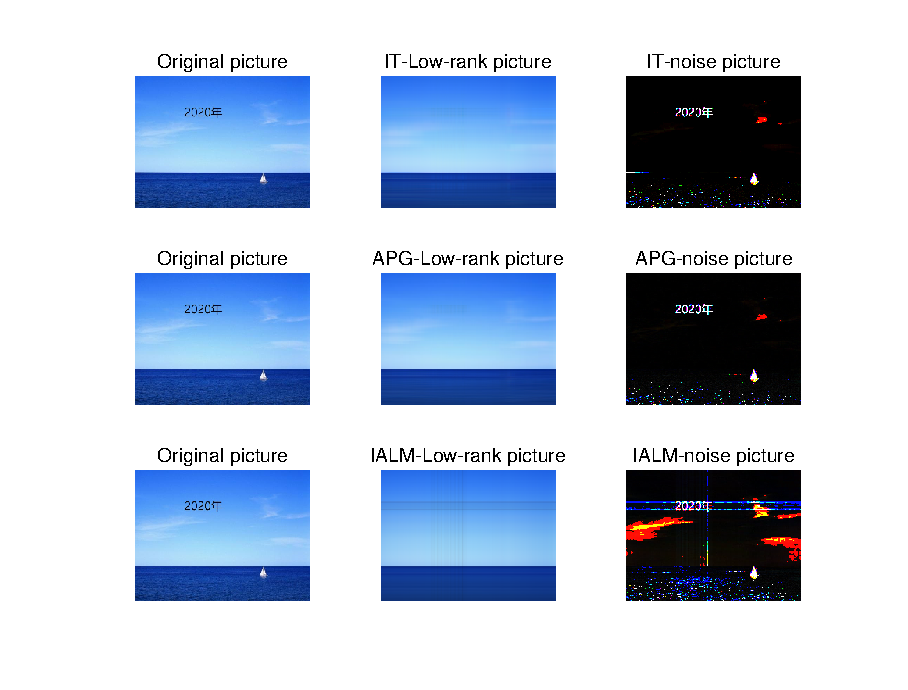
\includegraphics{Image Deblurring A.eps}
\caption{Image Deblurring A}
\label{1}
\end{figure}
\begin{figure}
\centering
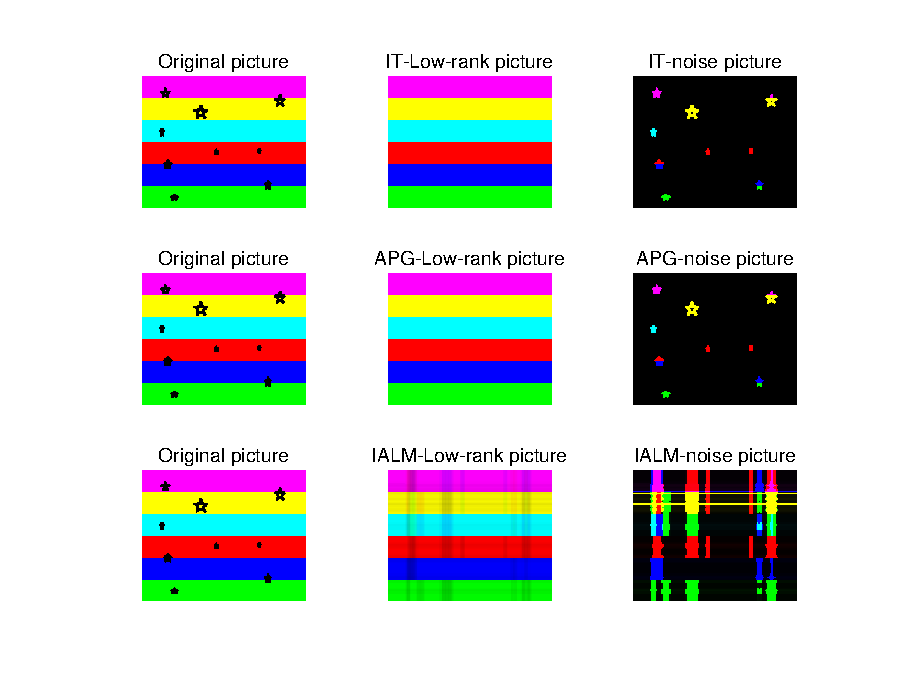
\includegraphics{Image Deblurring B.eps}
\caption{Image Deblurring B}
\label{2}
\end{figure}
\begin{figure}
\centering
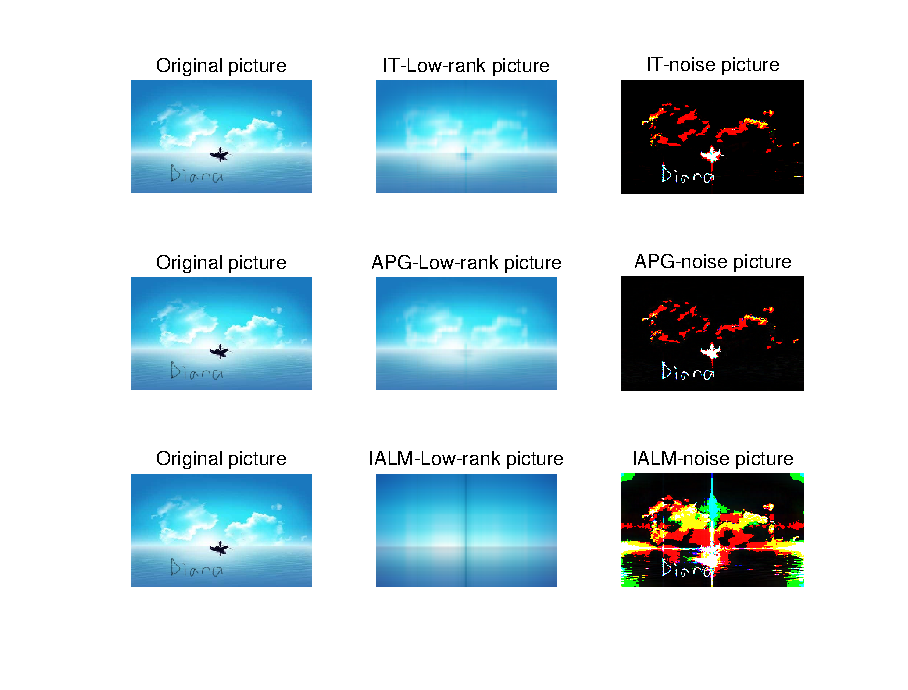
\includegraphics{Image Deblurring C.eps}
\caption{Image Deblurring C}
\label{3}
\end{figure} 

Some images have elements that can be seen as sparse and high-intensity noise, so we can separate them with the three algorithms above. See figure \ref{4}, \ref{5}, \ref{6}.
\begin{figure}
\centering
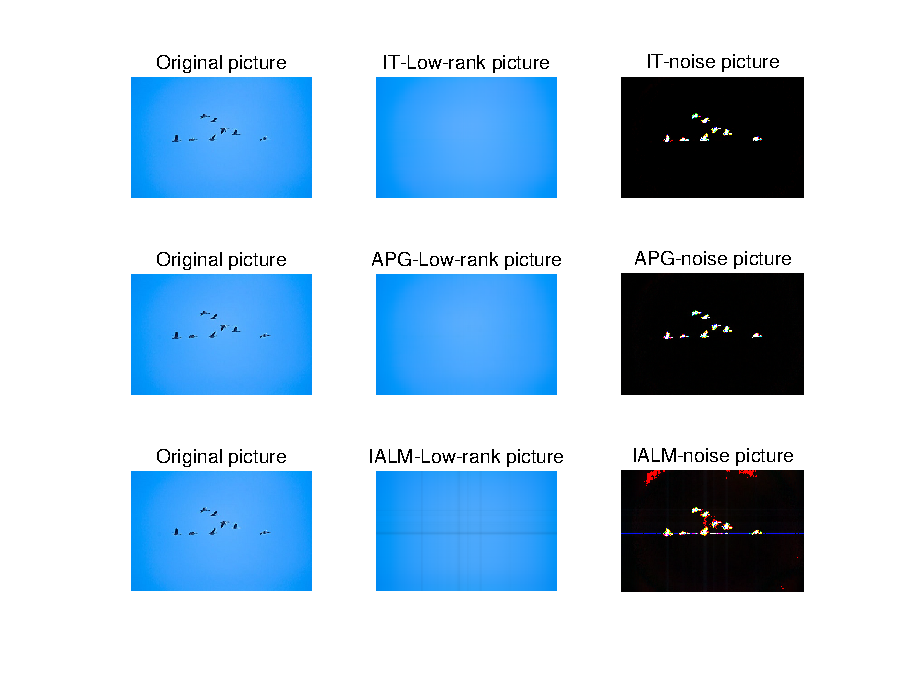
\includegraphics{Image Separation A.eps}
\caption{Image Separation A}
\label{4}
\end{figure}
\begin{figure}
\centering
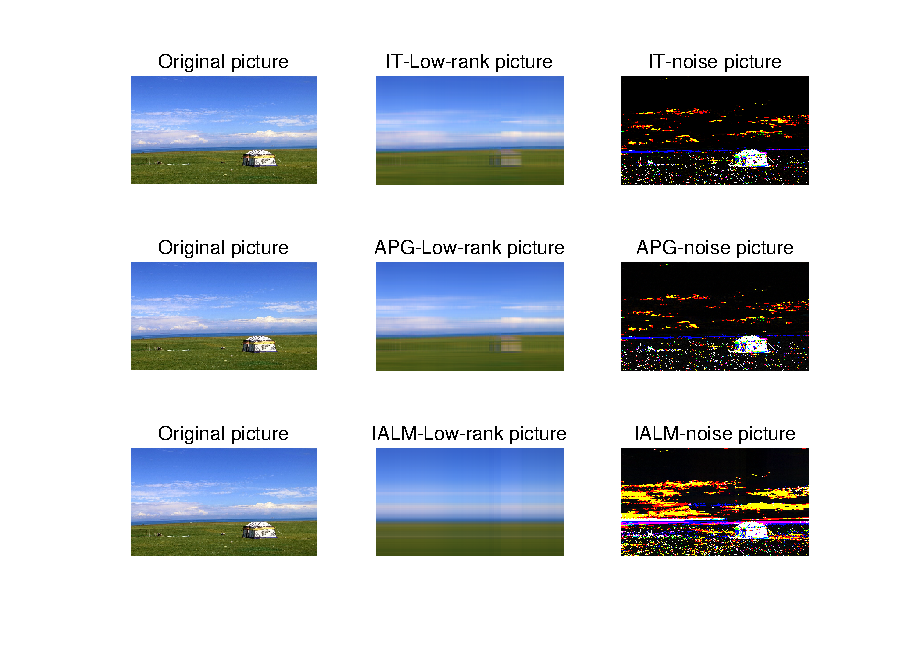
\includegraphics{Image Separation B.eps}
\caption{Image Separation B}
\label{5}
\end{figure}
\begin{figure}
\centering
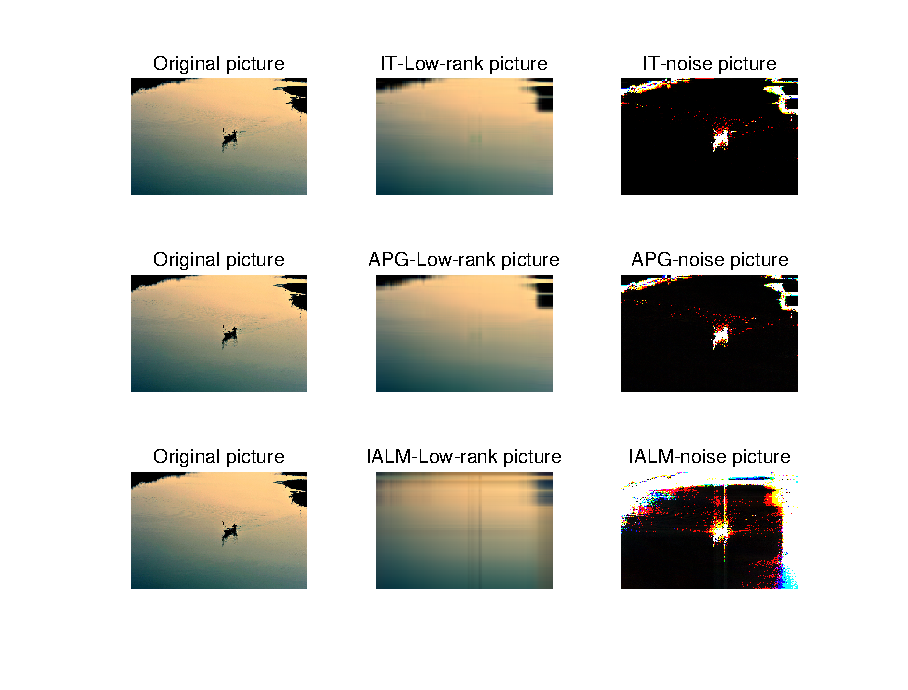
\includegraphics{Image Separation C.eps}
\caption{Image Separation C}
\label{6}
\end{figure} 

After observation, IT algorithm and APG algorithm are often more accurate than the low-rank matrix obtained by IALM algorithm, and the obtained sparse noise matrix is closer to the noise added later.
\begin{appendix}
    \renewcommand{\thechapter}{\Alph{chapter}.}
    \chapter{Reference For Test}
    \lstinputlisting{sto.m}
    \lstinputlisting{svto.m}
    \lstinputlisting{IT.m}
    \lstinputlisting{APG.m}
    \lstinputlisting{IALM.m}
    \lstinputlisting{project_image_inpainting.m}
    \lstinputlisting{image_separation.m}
\end{appendix}
\bibliography{reference}
\bibliographystyle{plain}
\end{document}
